
\section{Solution 1}
\label{sec:auswertung}

\begin{itemize}
    \item[1.]
    \begin{itemize}
        Zum Warmlaufen wird die Abbildung $N=30$ mal durchiteriert. Die Zahl wird relativ willkürlich gewählt, solle aber nicht zu niedrig sein.

        \item[a)]
        Überlegungen für das Maximale $r$:
        Werden die möglichen Werte $f(x)\equiv x_{n+1}$ gegen $x_n$ aufgetragen entstehen umgedrehte Parabeln, wobei die $x$-position des Maximums/Scheitelpunkts $r$-unabhägig ist:
        
        \begin{align}
            f'(x) & = r(1-2x) \overset{!}{=} 0 \\
            \Rightarrow x_0 & = 0.5 \\
            \Rightarrow f(x_0) & = r(x_0-x_0^2) \overset{!}{=} 1 \\
            \Rightarrow r & = 4
        \end{align}
        $r$ ist also maximal $4$.

        \item[b)]
        Es wird grafisch herausgefunden, dass $r \leq 3$ sein darf.
    \end{itemize}
    \item[2./3.]
    \begin{itemize}
        $r$ wird systematisch in Schritten $\Delta r = 0.001$ vatiiert. Jeder $r$- Wert erzeugt jeweilige Fixpunkte, welche dann in $r$-Abhängigkeit in ein Diagramm aufgetragen werden. 
        Es werden verschiedene Startwerte $x_0$ verwendet. 
        \item[a)]
        In den Tabellen \ref{tab:log} und \ref{tab:kub} sind die $r$-Werte angegeben, ab denen die Anzahl Fixpunkte größer als $64$ wird.
        \begin{table}[h]
            \centering
            \caption{Werte $r_{\infty}$ für die logistische Abbildung.}
            \label{tab:log}
            \sisetup{table-format=1.3}
            \begin{tabular}{S S}
                \toprule
                {$x_0$} & {$r_{\infty}$} \\
                \midrule
                0.1 & 3.853 \\
                0.3 & 3.632 \\
                0.5 & 3.889 \\
                0.7 & 3.632 \\
                0.9 & 3.732 \\
                
                \bottomrule
                
            \end{tabular}

        \end{table}


        \begin{figure}
            \begin{subfigure}{.6\textwidth}
                \centering

                \subcaption{$x_0 = 0.5$}
                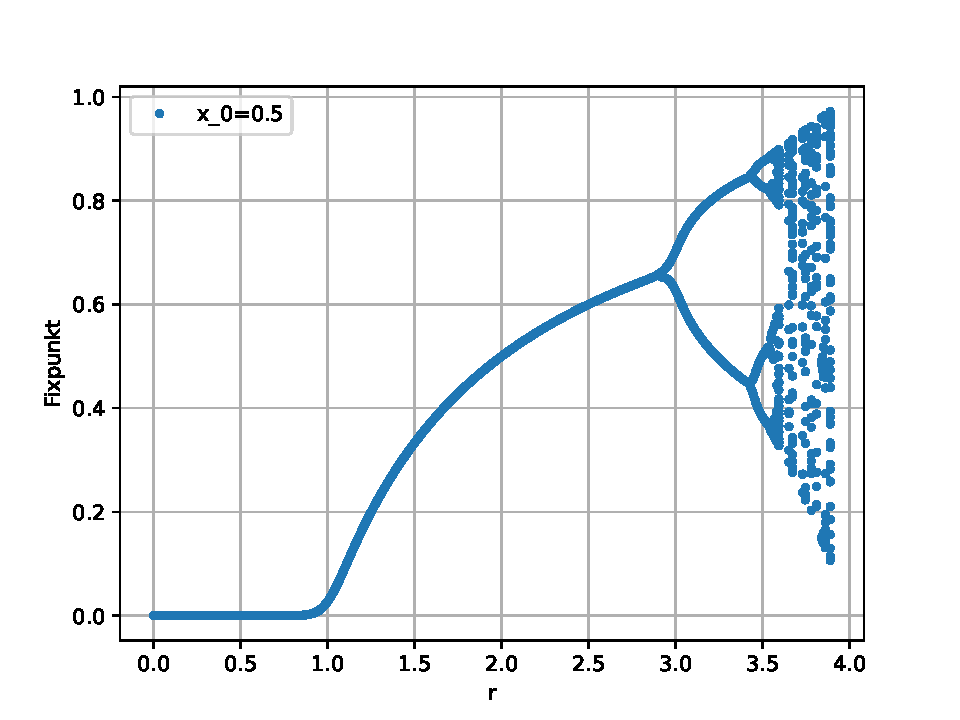
\includegraphics[width=.9\linewidth]{images/Bif_log2.pdf}
            \end{subfigure}
            \begin{subfigure}{.6\textwidth}
                \centering
                \subcaption{$x_0 = 0.1$}
                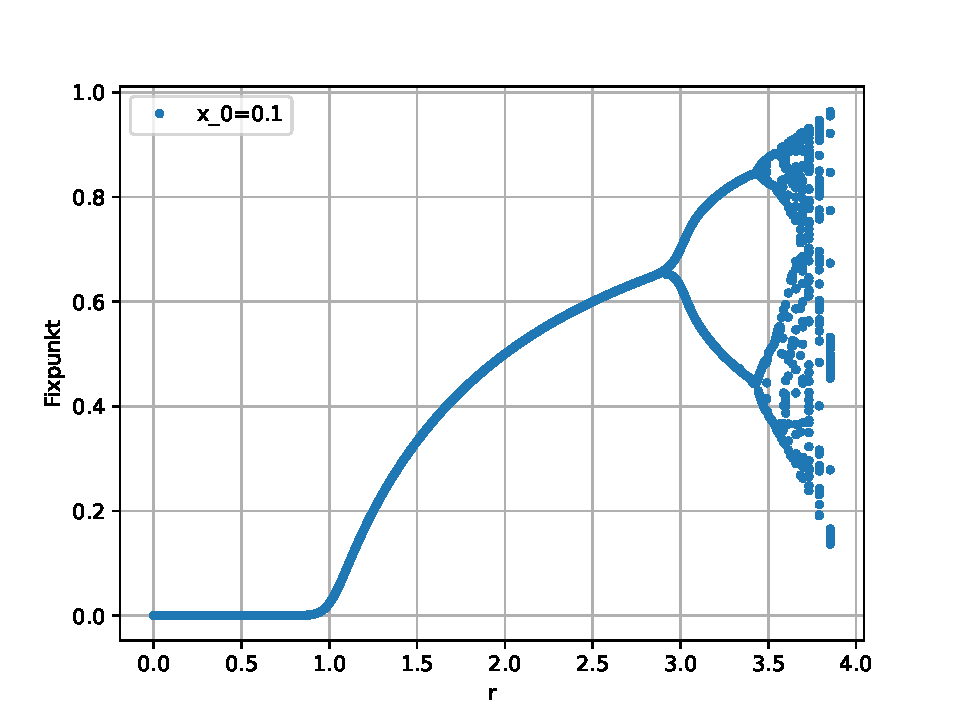
\includegraphics[width=.9\linewidth]{images/Bif_log0.pdf}
                \end{subfigure}
            \caption{Bifurkationsdiagramm der logistischen Abbildung. }
        \end{figure}
        \item[b)]

        \begin{table}[h]
            \centering
            \caption{Werte $r_{\infty}$ für die kubische Abbildung.}
            \label{tab:kub}
            \sisetup{table-format=1.3}
            \begin{tabular}{S S}
                \toprule
                {$x_0$} & {$r_{\infty}$} \\
                \midrule
                0.1 & 2.421 \\
                0.3 & 2.102 \\
                0.5 & 2.457 \\
                0.7 & 2.346 \\
                0.9 & 2.323 \\
                \bottomrule
                
            \end{tabular}

        \end{table}

        \begin{figure}
            \begin{subfigure}{.6\textwidth}
                \centering
                \subcaption{$x_0 = 0.5$}
                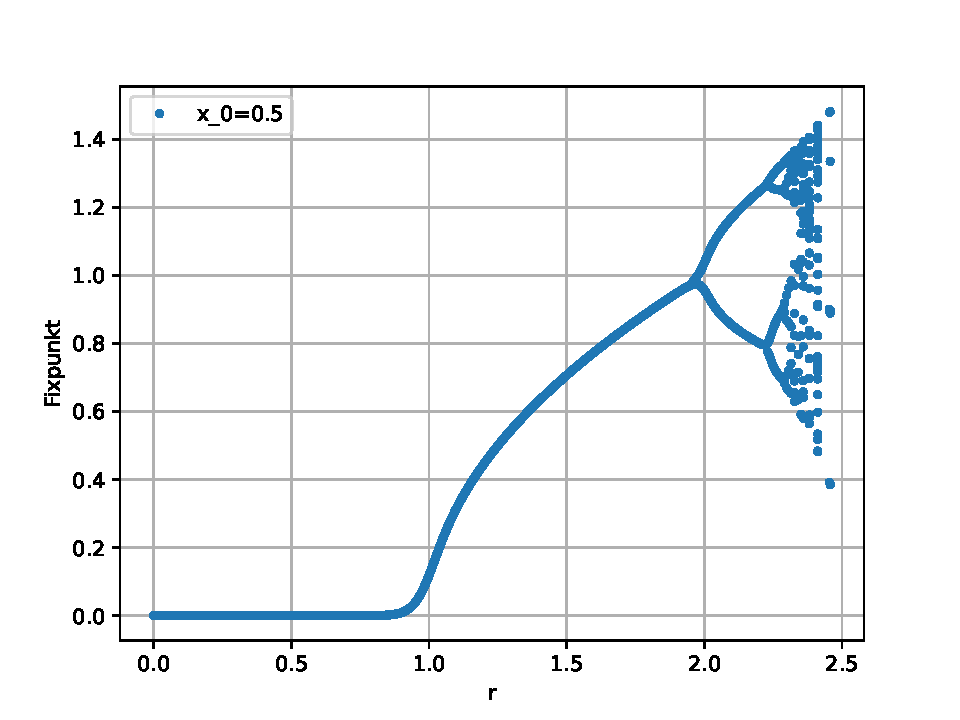
\includegraphics[width=.9\linewidth]{images/Bif_kub2.pdf}
            \end{subfigure}
            \begin{subfigure}{.6\textwidth}
                \centering
                \subcaption{$x_0 = 0.1$}
                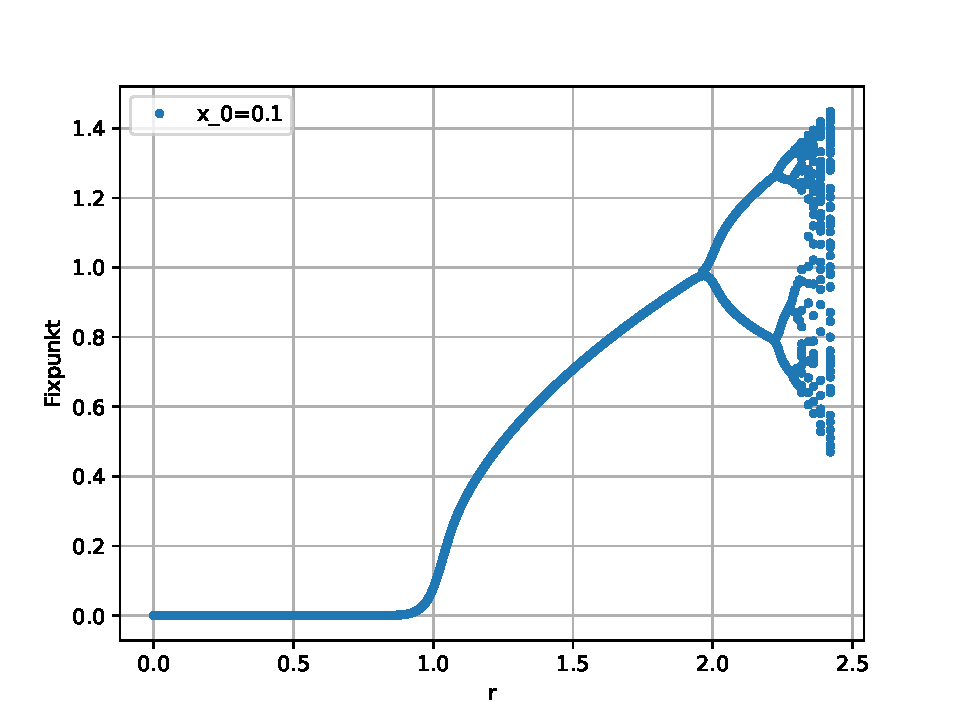
\includegraphics[width=.9\linewidth]{images/Bif_kub0.pdf}
                \end{subfigure}
            \caption{Bifurkationsdiagramm der kubischen Abbildung. }

        \end{figure}
    \end{itemize}

    Leider hat das bestimmen der Feigenbaumkonstante nicht gut funktioniert. 
    Im Terminal werden beim Ausführen des Codes die $r$-Werte ausgegeben, bei denen sich die Anzahl Fixpunkte gegenüber dem vorherigen $r$ ändern.
    Leider kommen da nicht so sinnvolle Anzahlen von Fixpunkten bei rum... 

\end{itemize}


\section{Solution 2}
\label{sec:auswertung}
    \begin{itemize}
        \item[a)]
            In the second exercise we were asked to solve the Lorentz equations 
            \begin{align*}
                \dot{X} = & -\sigma X + \sigma Y \\
     ̇           \dot{Y} = & -XZ + rX - Y \\
     ̇           \dot{Z} = & XY - bZ
            \end{align*}
            with the fourth order Runge-Kutta scheme.
            The implementation can be found in file "2.cpp".
            The parameters $r, \sigma$ and $b$ were given as:
            \begin{align*}
                r = & 20 \,\text{or}\, 28\\
                \sigma = & 10 \\
                b = & 8/3
            \end{align*}
            In the following plots one can clearly see that a change in the starting parameter such as $r$ results in a different behaviour.
            One gives a stable orbit around an attractor, the other falls into the attractor.
            Other parameters show even different behaviour.
            However, the starting position does not influecs the trajectory.
        \item[b)]
            After the implementation we were asked to visualize our solution.
            This should be done in three ways
            \begin{itemize}
                \item[1.]
                    First as a projection of the trajectory on the xy-plane.
                    \FloatBarrier
                    \begin{figure}
                        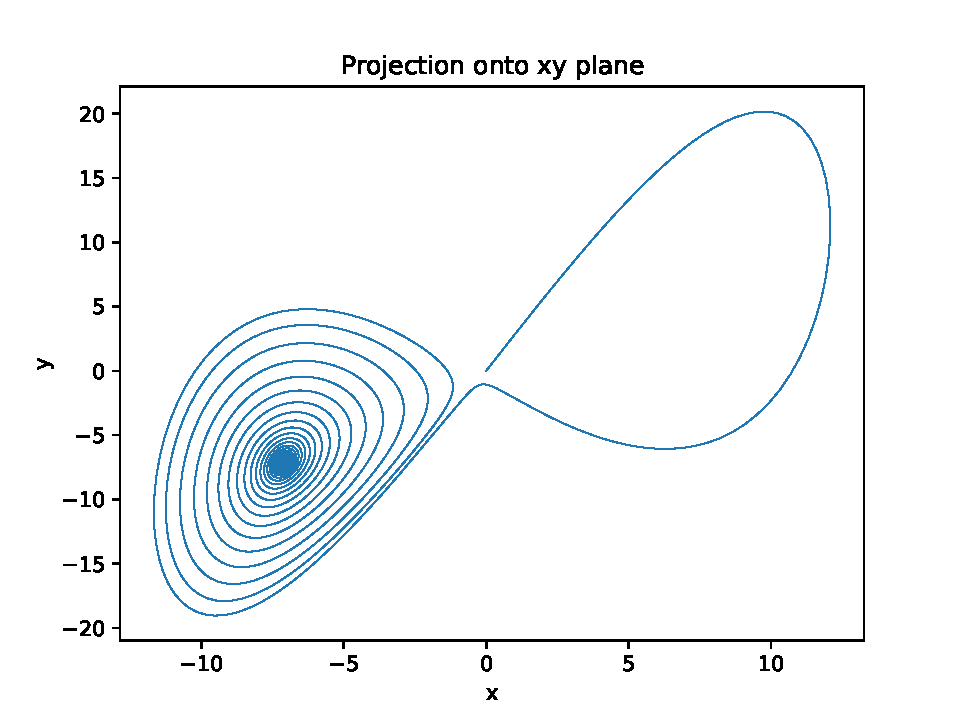
\includegraphics[width=\textwidth]{images/Lorentz_r_20_projection.pdf}
                        \caption{The projection of the trajectory onto the xy-plane with the starting parameter $r=20$.}
                    \end{figure}
                    \begin{figure}
                        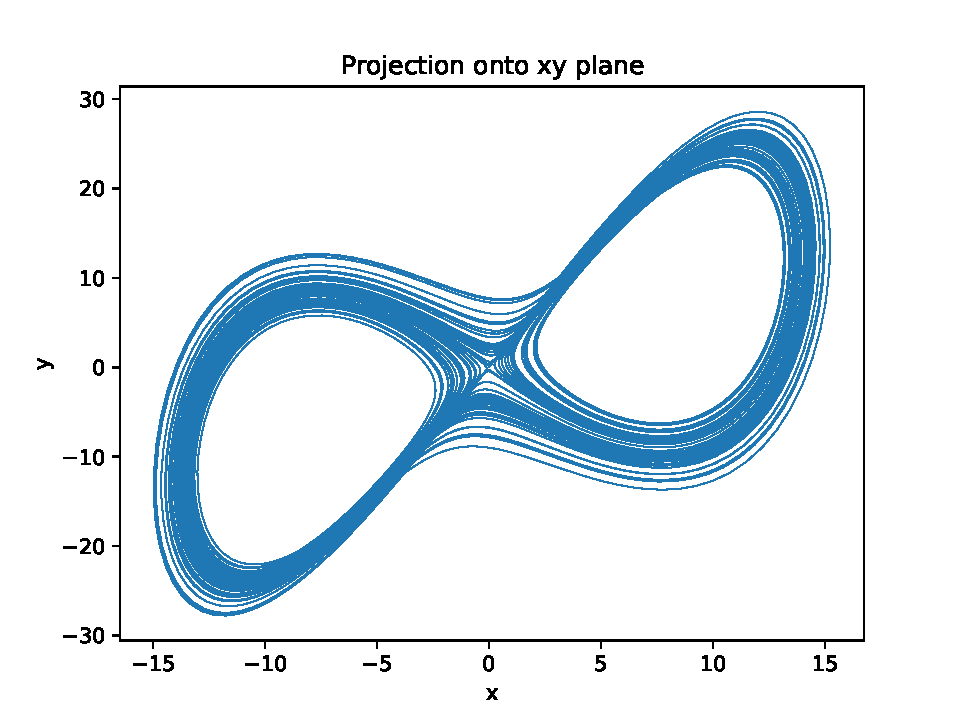
\includegraphics[width=\textwidth]{images/Lorentz_r_28_projection.pdf}
                        \caption{The projection of the trajectory onto the xy-plane with the starting parameter $r=28$.}
                    \end{figure}
                    \FloatBarrier
                \item[2.]
                    As a Poincare slice at $Z=20$ with the condition that $\dot{Z} < 0$.
                    We tested for this condition by subtracting the $\vec{f}(t_i)$ with $\vec{f}(t_{i+1})$. 
                    If the result is basically a linear interpolation between point $\vec{f}(t_i)$ and $\vec{f}(t_{i+1})$.
                    We then plotted all points that forfill the two conditions onto a xy-plane.
                    \FloatBarrier
                    \begin{figure}
                        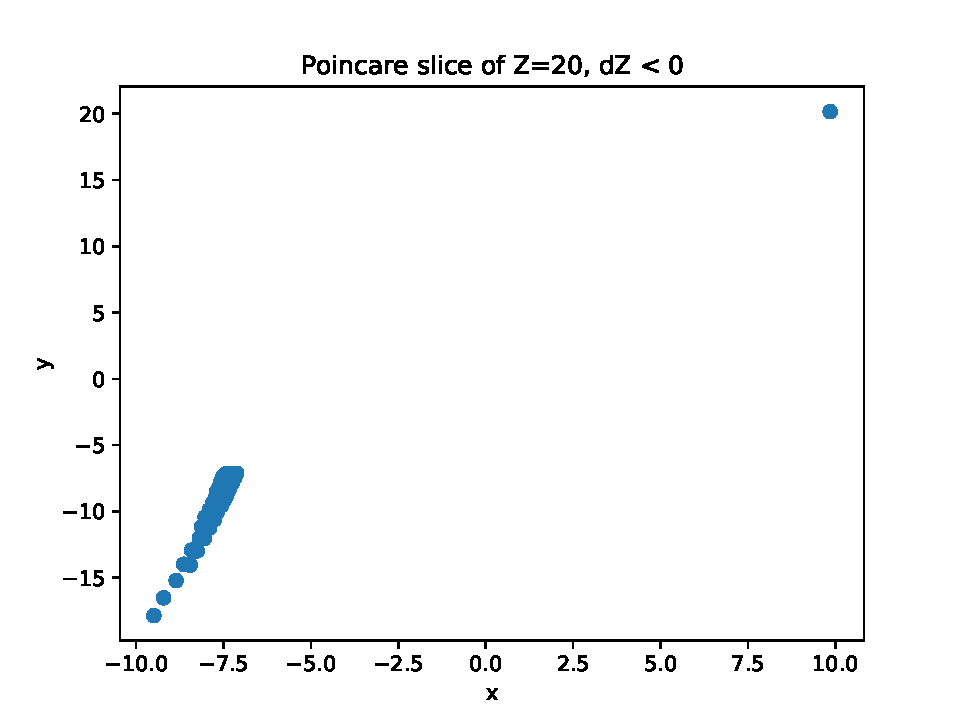
\includegraphics[width=\textwidth]{images/Lorentz_r_20_slice.pdf}
                        \caption{The Poincare slice of the trajectory onto the xy-plane with the starting parameter $r=20$.}
                    \end{figure}
                    \begin{figure}
                        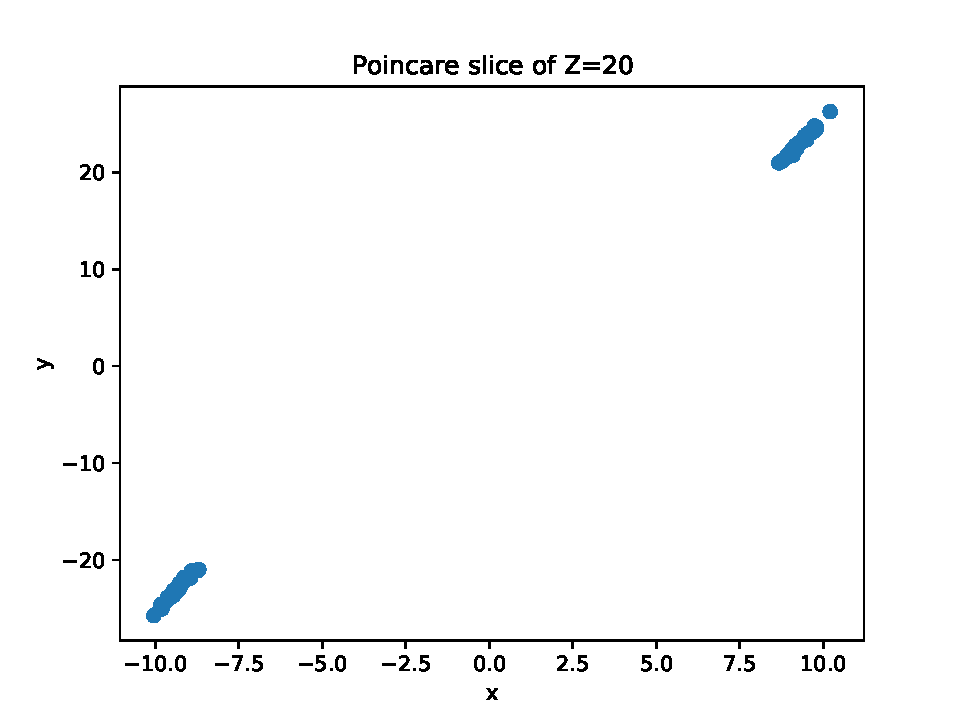
\includegraphics[width=\textwidth]{images/Lorentz_r_28_slice.pdf}
                        \caption{The Poincare slice of the trajectory onto the xy-plane with the starting parameter $r=28$.}
                    \end{figure}
                    \FloatBarrier
                \item[3.]
                    For the last part we plotted the whole xyz-trajectory onto a 3d-plot.
                    \FloatBarrier
                    \begin{figure}
                        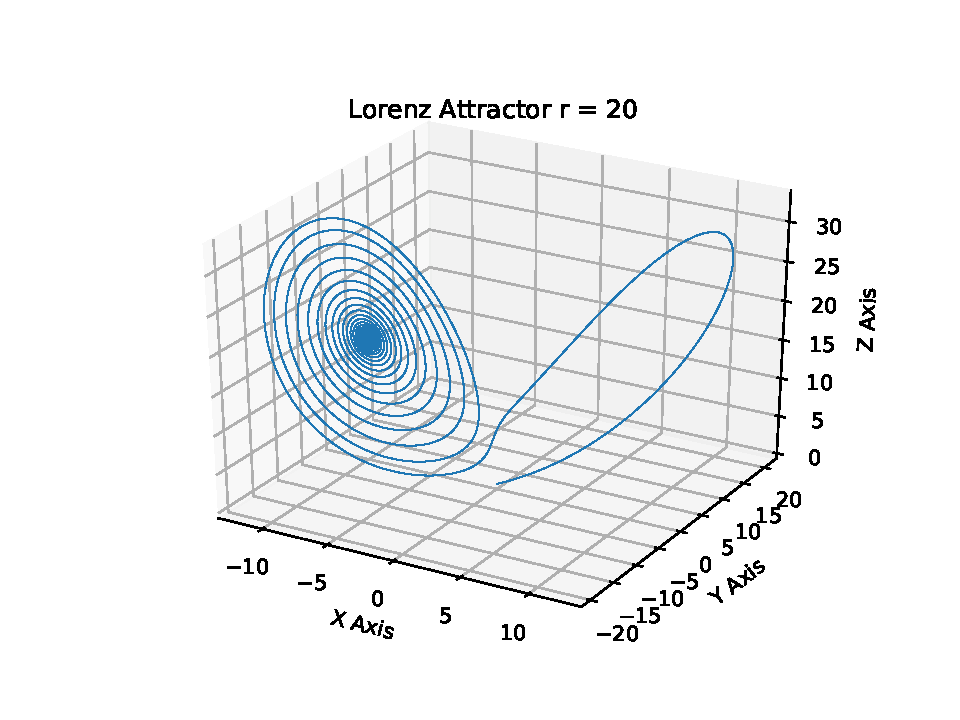
\includegraphics[width=\textwidth]{images/Lorentz_r_20_3d.pdf}
                        \caption{The 3d-Plot of the trajectory with the starting parameter $r=20$.}
                    \end{figure}
                    \begin{figure}
                        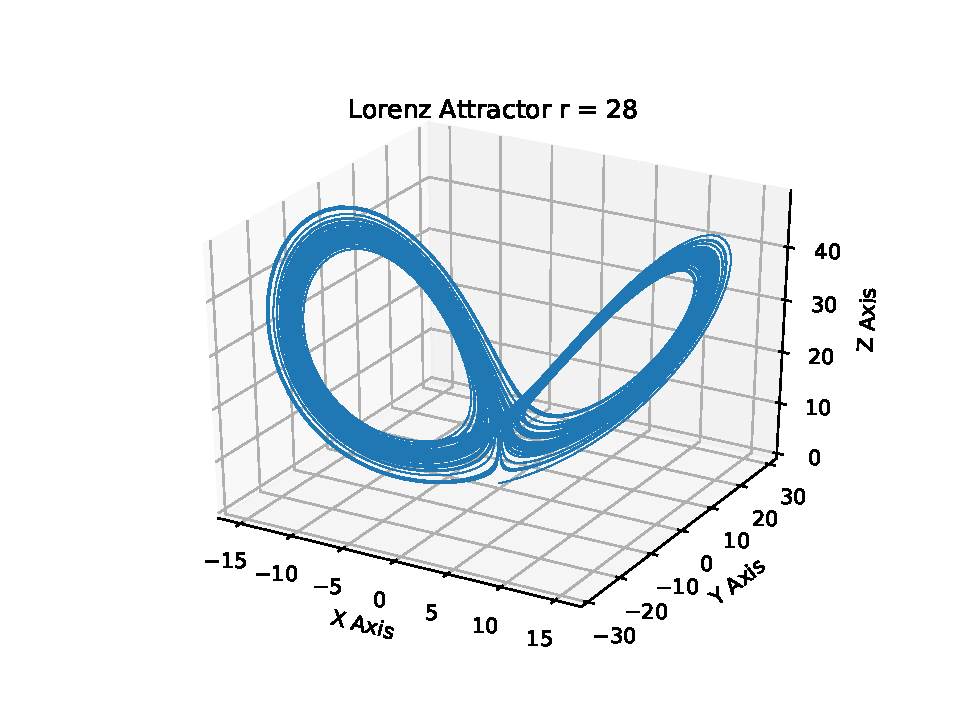
\includegraphics[width=\textwidth]{images/Lorentz_r_28_3d.pdf}
                        \caption{The 3d-Plot of the trajectory with the starting parameter $r=28$.}
                    \end{figure}
            \end{itemize}
\end{itemize}              